\documentclass[8pt,landscape]{article}

% PACKAGES
\usepackage[letterpaper, margin=0.1in]{geometry}
\usepackage{amsmath, amssymb, geometry}
\usepackage{multicol}
\usepackage{setspace}
\usepackage{sectsty}
\usepackage{verbatim}
\usepackage{graphicx}
\usepackage{xcolor}
\usepackage{listings}
\usepackage{enumitem}
\usepackage{booktabs} 

% Colors
\definecolor{myred}{RGB}{204, 0, 0} 
\definecolor{mygray}{RGB}{240, 240, 240} 
\setlist[itemize]{
    noitemsep,  
    topsep=0pt,  
    partopsep=0pt, 
    parsep=0pt, 
    leftmargin=*, 
    labelsep=0.3em, 
}

% LISTINGS SETUP
\lstset{
  basicstyle=\ttfamily\tiny\color{black},
  backgroundcolor=\color{mygray},
  frame=single,
  frameround=tttt,
  framesep=1pt,        
  rulecolor=\color{black!20},
  breaklines=true,
  columns=fullflexible,
  showstringspaces=false,
  commentstyle=\color{gray},
  keywordstyle=\color{blue!80!black},
  stringstyle=\color{myred},
  xleftmargin=2pt,     
  xrightmargin=2pt,    
  aboveskip=1pt,       
  belowskip=1pt,       
}

% FORMATTING
\setstretch{0.8} 
\setlength{\parindent}{0pt}
\setlength{\parskip}{0pt}

\makeatletter
\renewcommand{\section}{\@startsection{section}{2}{0pt}%
    {0.1ex}{0.1ex}{\fontsize{8}{9}\bfseries\color{red}}} 
\makeatother

\makeatletter
\renewcommand{\subsection}{\@startsection{subsection}{2}{0pt}%
    {0.1ex}{0.1ex}{\fontsize{7}{8}\bfseries\color{blue}}} 
\makeatother

\newcommand{\code}[1]{\textcolor{myred}{\texttt{#1}}}
\newcommand{\smalltext}[1]{{\fontsize{7}{8}\selectfont\sloppy #1\par}}

\begin{document}
\fontsize{7}{8}\selectfont 
\pagestyle{empty}
\begin{multicols}{3}

\section{Word Embeddings (Lec 5)}
\begin{lstlisting}[language=python]
def euclidean_distance(a, b): # Euclidean distance: smaller distance - more similar
    return np.linalg.norm(a - b)
def dot_product_similarity(a, b):# Dot product similarity: larger dot product - more similar 
    return np.dot(a, b)
def cosine_similarity(a, b):# Cosine similarity: larger similarity score - more similar
    return dot(a, b) / (norm(a) * norm(b))
v1 = np.array([2, 4, 3])
v2 = np.array([5, 1, 0])
print(f"Euclidean Distance: {euclidean_distance(v1, v2):.4f}")
print(f"Dot Product Similarity: {dot_product_similarity(v1, v2):.4f}")
print(f"Cosine Similarity: {cosine_similarity(v1, v2):.4f}")
\end{lstlisting}

\subsection{Term - Term Co-occurrence Context}
\smalltext{
    \textbf{One-hot:} $|V|$ dimensions. Sparse. No inherent notion of relationship between words and the dot product between similar and non-similar words is zero.
    \textbf{Diagonal Zeroes:} The diagonal entries are zero because we typically do not consider a word to be its own context in these models.
    The operation is $vector(b) - vector(a) + vector(c)$. The system then searches for the word vector closest to this result.
    go through a corpus of text, keeping a count of all of the words that appear in context of each word (within a window). The similarity is calculated using dot products between word vectors.

}

\subsection{Word2Vec - Skip Gram - Gensim}
\smalltext{
    Dense Representations. NN model to obtain short and dense representations of words. A simple architecture with 1. Input layer 2. linear hidden layer (without any activation function) 3. Output layer with softmax. Goal is learn meaningful weights (meaningful representation of the input) in the process.
    Given a target word (i.e., center word) word, predict context words (i.e., surrounding words). 
    \textbf{Negative sampling:} Instead of computing probabilities for all words, the model updates only a small number of negative samples (randomly selected words that are unlikely to be in the context).
    \textbf{Hierarchical softmax:} Instead of computing softmax over the entire vocabulary, words are arranged in a binary tree structure, allowing predictions to be made in $Log(V)$ time instead of $O(V)$.
}
\smalltext{
    \textbf{Pre-trained Embeddings}
    \textbf{word2vec} trained on several corpora using the word2vec algorithm.We use pre-trained embeddings (like GloVe or Word2Vec) because training them from scratch requires massive datasets and high computational power; pre-trained models capture general semantic relationships that are difficult to learn on smaller, domain-specific data.
    \textbf{fastText Advantage:} It is particularly useful if your corpus updates frequently with unknown words, as it uses subword information (character n-grams) to create embeddings for words not seen during training.
    \textbf{Implicit biases and stereotypes in word embeddings}: Embeddings reflect gender stereotypes present in broader society.
    They may also amplify these stereotypes because of their widespread usage.

}
\begin{lstlisting}[language=python]
    google_news_vectors = api.load("word2vec-google-news-300")
    model = Word2Vec(sentences, vector_size=10, window=5, min_count=1) # train word2vec model
    model.wv.most_similar("cat")
\end{lstlisting}
\smalltext{
\textbf{Skip-gram:} input = target word, output = surrounding context words

\textbf{CBOW:} input = context words, output = target word

A problem with generating word embeddings: \textbf{Social bias} can show up in the embedding space.
}

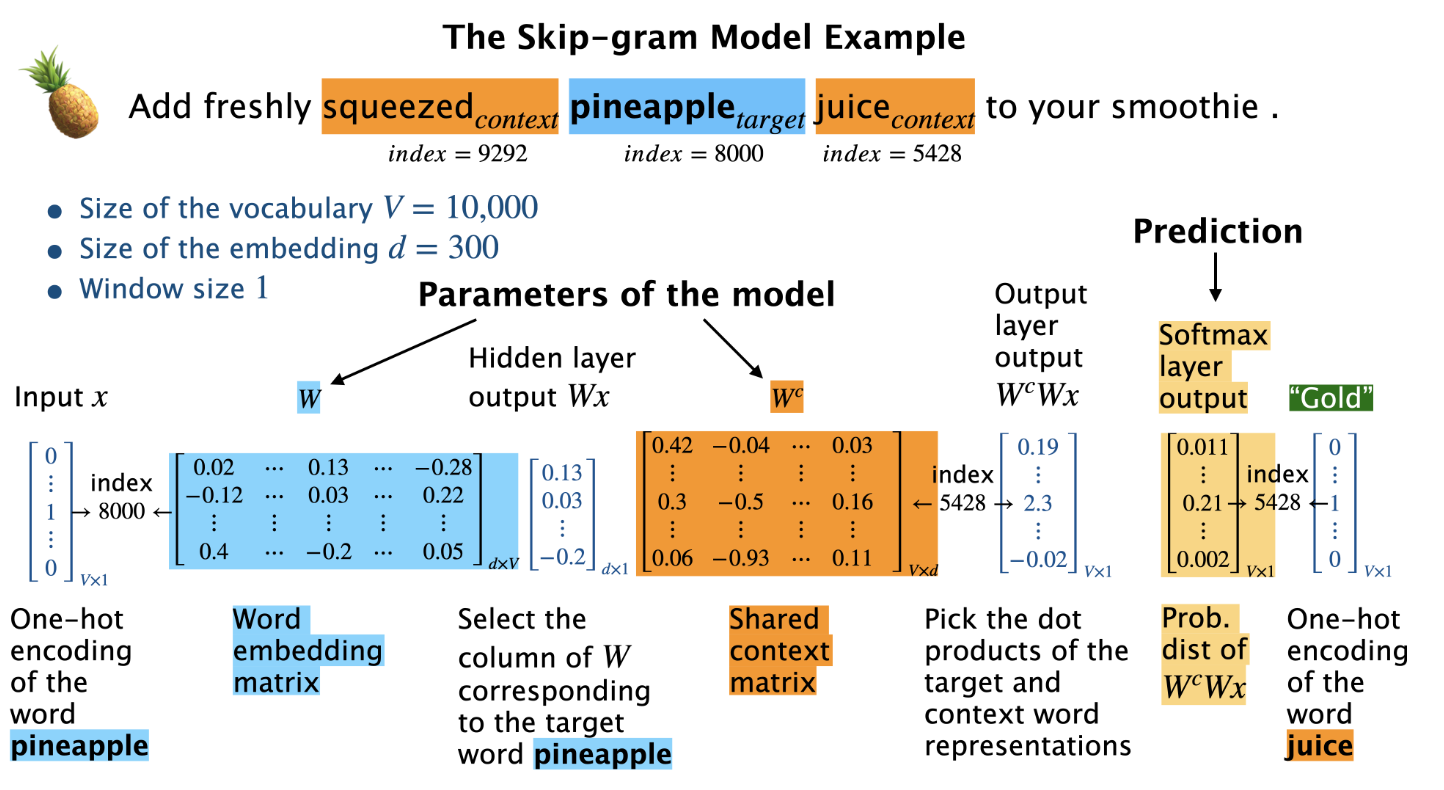
\includegraphics[width=1\linewidth, height=3cm]{skip-gram.png}

\section{Latent Semantic Analysis LSA $X_{n \times d} \approx Z_{n \times k} W_{k \times d}$}
\smalltext{
$n$ number of documents, $k$ number of topics, $d$ number of features, $Z$ is document topic assignments, $W$ is topic-word assignments.
LSA TruncatedSVD for matrix factorization using SVD (without centering the data).  
\textbf{The Role of Centering:} Before factorizing, we subtract the global mean, user bias, and item bias. This ensures the model learns the interactions (latent features) rather than just the fact that some users are "easy raters" or some movies are "generally popular."
\textbf{Advantage: }
The idea is to reduce the dimensionality of the data to extract some semantically meaningful components.
\textbf{Disadvantage: }
Topics are not probability distributions over words.
Documents are not explicitly modeled as mixtures of topics.
There is no generative process explaining how words arise.
Not Probabilistic generative model hence we use LDA.
}

\section{Latent Dirichlet Allocation LDA}
\smalltext{
LSA disadvantage is \textbf{advantage}. we assume each document has a distribution over topics and each topic has a distribution over words. 
LDA is a Bayesian probabilistic generative model with Dirichlet priors, we compute the posterior distribution over these latent variables. However, this posterior has no closed-form solution. So we rely on approximate inference methods.

1. The Priors - (Dirichlet Distributions) - Document-Topic Prior ($\alpha$) Represents our prior belief about the distribution of topics within documents.

2. The Likelihood - Multinomial distribution - the topic assignments - clusters u want

\textbf{Why generative?}because we can generate words from this model. Its discrete because of count of words.

\textbf{how dif from k-means:}In clustering with K-Means, documents are grouped based on a similarity measure, and each document is assigned to a single cluster. In contrast, topic modeling produces distributions over words for each topic, as well as distributions over topics per document.

LDA is a soft clustering technique. While K-Means assigns a document to exactly one cluster, LDA produces a distribution, meaning a document can be a mixture of several topics.
The Dirichlet controls how mixed or concentrated a probability distribution is.

\textbf{Case 1: Small $\alpha$=0.1} - Distributions are sparse and peaked.
A document is mostly about one topic.
Topics are specialized.
Fewer mixtures.

\textbf{Case 2: Large $\alpha$=10} - Distributions are smooth and spread out.
A document mixes many topics evenly.
Topics are less distinct.
More mixing.
}

\textbf{Gibbs sampling (accurate but slow; good for small datasets)}
\smalltext{
    Markov Chain Monte Carlo (MCMC) algorithm used to estimate the posterior distribution of hidden variables (topic assignments) that are otherwise computationally intractable to calculate directly.
}
\subsection{Topic Modeling Pipeline}
\smalltext{
   \textbf{1. Corpus Preprocessing:} Normalization via case-folding and punctuation removal. Token filtration involves $n$-length thresholds and frequency pruning (e.g., \code{filter\_extremes}). \textbf{Lemmatization} reduces inflected forms to morphological roots; \textbf{POS tagging} can restrict the feature space to specific grammatical categories (e.g., Nouns/Adjectives) to enhance semantic density.
   
   \textbf{2. Model Training (Gensim/sklearn):} Construction of a \textbf{Document-Term Matrix (DTM)}. Using \code{corpora.Dictionary}, tokens are mapped to indices (\code{token2id}) and documents are transformed into sparse \textbf{Bag-of-Words (BoW)} vectors (\code{doc2bow}). Key hyperparameters: $K$ (\code{num\_topics}) and \code{passes} (epochs).
   
   \textbf{3. Evaluation \& Interpretation:}
   \begin{itemize}
       \item \textbf{Qualitative Analysis:} "Eyeballing" top-$N$ words per topic or documents with high posterior probability $P(z|d)$.
       \item \textbf{Human Judgments:} Assessing "story coherence" or \textbf{Word Intrusion} tests. In Intrusion, an "outlier" word from a distal topic is inserted into a top-word set; model quality is measured by the human ability to identify the intruder (e.g., \textit{dentist, appointment, \textbf{mom}, doctor}).
       \item \textbf{Extrinsic Evaluation:} Benchmarking topics as downstream features (e.g., in Sentiment Analysis) to see if they improve predictive accuracy.
       \item \textbf{Quantitative Metrics (Coherence):} \code{CoherenceModel} measures semantic similarity between the most probable words in a topic. Scores range from $[-1, 1]$, where higher values indicate stronger semantic interpretability.
   \end{itemize}
}

\section{Recommender Systems: Introduction}
\smalltext{
Recommender systems mitigate \textbf{information overload} by filtering large item spaces to suggest products/services based on predicted consumption. They optimize the discovery process by mapping user preferences to item attributes or behavioral patterns.
}
\smalltext{
\begin{itemize}
    \item \textbf{Collaborative Filtering (CF):} Unsupervised approach leveraging user-item interaction matrices to discover \textbf{latent features}.
    \item \textbf{Content-based:} Supervised learning utilizing explicit user/item metadata (e.g., genre, demographics) to predict affinities.
    \item \textbf{Hybrid:} Ensemble methods combining CF and Content-based signals to mitigate individual algorithmic weaknesses.
\end{itemize}
}
\subsection{Ethics and Filter bubles}
\smalltext{
Exploitation-heavy algorithms lead to \textbf{Filter Bubbles}, narrowing user exposure to diverse content. Ethical risks include the "Cold Start" problem (new users/items), data privacy concerns, and the potential for maximizing engagement at the cost of radicalization or misinformation.
Algorithms optimizing solely for engagement can catalyze extremist rabbit holes and political polarization. Designers must evaluate the societal impact and "Filter Bubble" effects before deployment.
}

\subsection{The Utility Matrix ($Y$)}
\smalltext{
An $N \times M$ matrix where $N$ = users and $M$ = items. $Y$ is typically \textbf{highly sparse} ($<1\%$ density). The objective is \textbf{Matrix Completion}: predicting unobserved entries $\hat{y}_{ij}$ to recommend high-value items.
}
\textbf{Evaluation Metrics}
\smalltext{
Performance is validated via \textbf{(RMSE)}or \textbf{(MSE)}.
}
\subsection{Baseline Imputation}
\smalltext{
Are critical because they serve as a "sanity check." If a complex Collaborative Filtering model cannot beat a simple average, it is not adding value.
\begin{itemize}
    \item \textbf{Simple Averages:} Global $\mu$, per-user $\mu_i$, or per-item $\mu_j$.
    \item \textbf{K-Nearest Neighbors (KNN):} Imputing missing values based on the $k$ most similar users/items in the training manifold.
\end{itemize}
}
% \begin{lstlisting}[language=python]
% from sklearn.impute import KNNImputer
% imputer = KNNImputer(n_neighbors=2) # Impute missing values based on spatial proximity
% train_mat_imp = imputer.fit_transform(train_mat)
% \end{lstlisting}

\section{Collaborative Filtering \& SVD}
\smalltext{
   SVD Limitation: You cannot run standard SVD on a utility matrix with missing values because the math is undefined for incomplete matrices. To use it, you must first "impute" or fill the missing values (often with the global or user mean).
}
\textbf{Matrix Factorization (MF)}
\smalltext{
The predicted rating is the dot product: $\hat{y}_{ij} = w_j^T z_i$.
}
\textbf{Regularized Objective Function:}
\smalltext{
Since standard SVD is undefined for missing data, CF minimizes the squared error over \textbf{observed ratings} $R$ with $L_2$ regularization.
}
\textbf{Incorporating Biases:}
\smalltext{
To account for systematic variations (e.g., "easy" raters or "popular" items), we add bias terms:
Where $\beta$ is global mean, $\beta_i$ is user bias, and $\beta_j$ is item bias.
}
\section{Implementation: Surprise Library}
\smalltext{
The \code{surprise} library uses Stochastic Gradient Descent (SGD) to minimize the regularized loss for SVD models.
}
\textbf{Problem Definition}
\smalltext{
The objective is to suggest items based on latent preference. Formulated as a \textbf{matrix completion} problem using a utility matrix $Y_{N \times M}$ encoding interactions between $N$ users and $M$ items. $Y$ is typically sparse ($<1\%$ density).
}
\smalltext{
\begin{itemize}
    \item \textbf{Collaborative Filtering (CF):} Leverages social signals/past agreement. Maps users/items to latent factor spaces $Z$ and $W$.
    \item \textbf{Content-based Filtering:} Supervised learning using intrinsic item features to predict ratings.
    \item \textbf{Hybrid:} Weighted ensembles or cascaded models combining CF and content signals.
\end{itemize}
}

\subsection{Dot Product vs. Cosine Similarity}
\smalltext{
\textbf{Dot Product} ($u \cdot v = \|u\|\|v\|\cos\theta$) is sensitive to vector magnitude, favoring "popular" items with high-norm embeddings. \textbf{Cosine Similarity} ($\frac{u \cdot v}{\|u\|\|v\|}$) normalizes by magnitude, measuring only angular displacement. This improves diversity by reducing popularity bias.
}
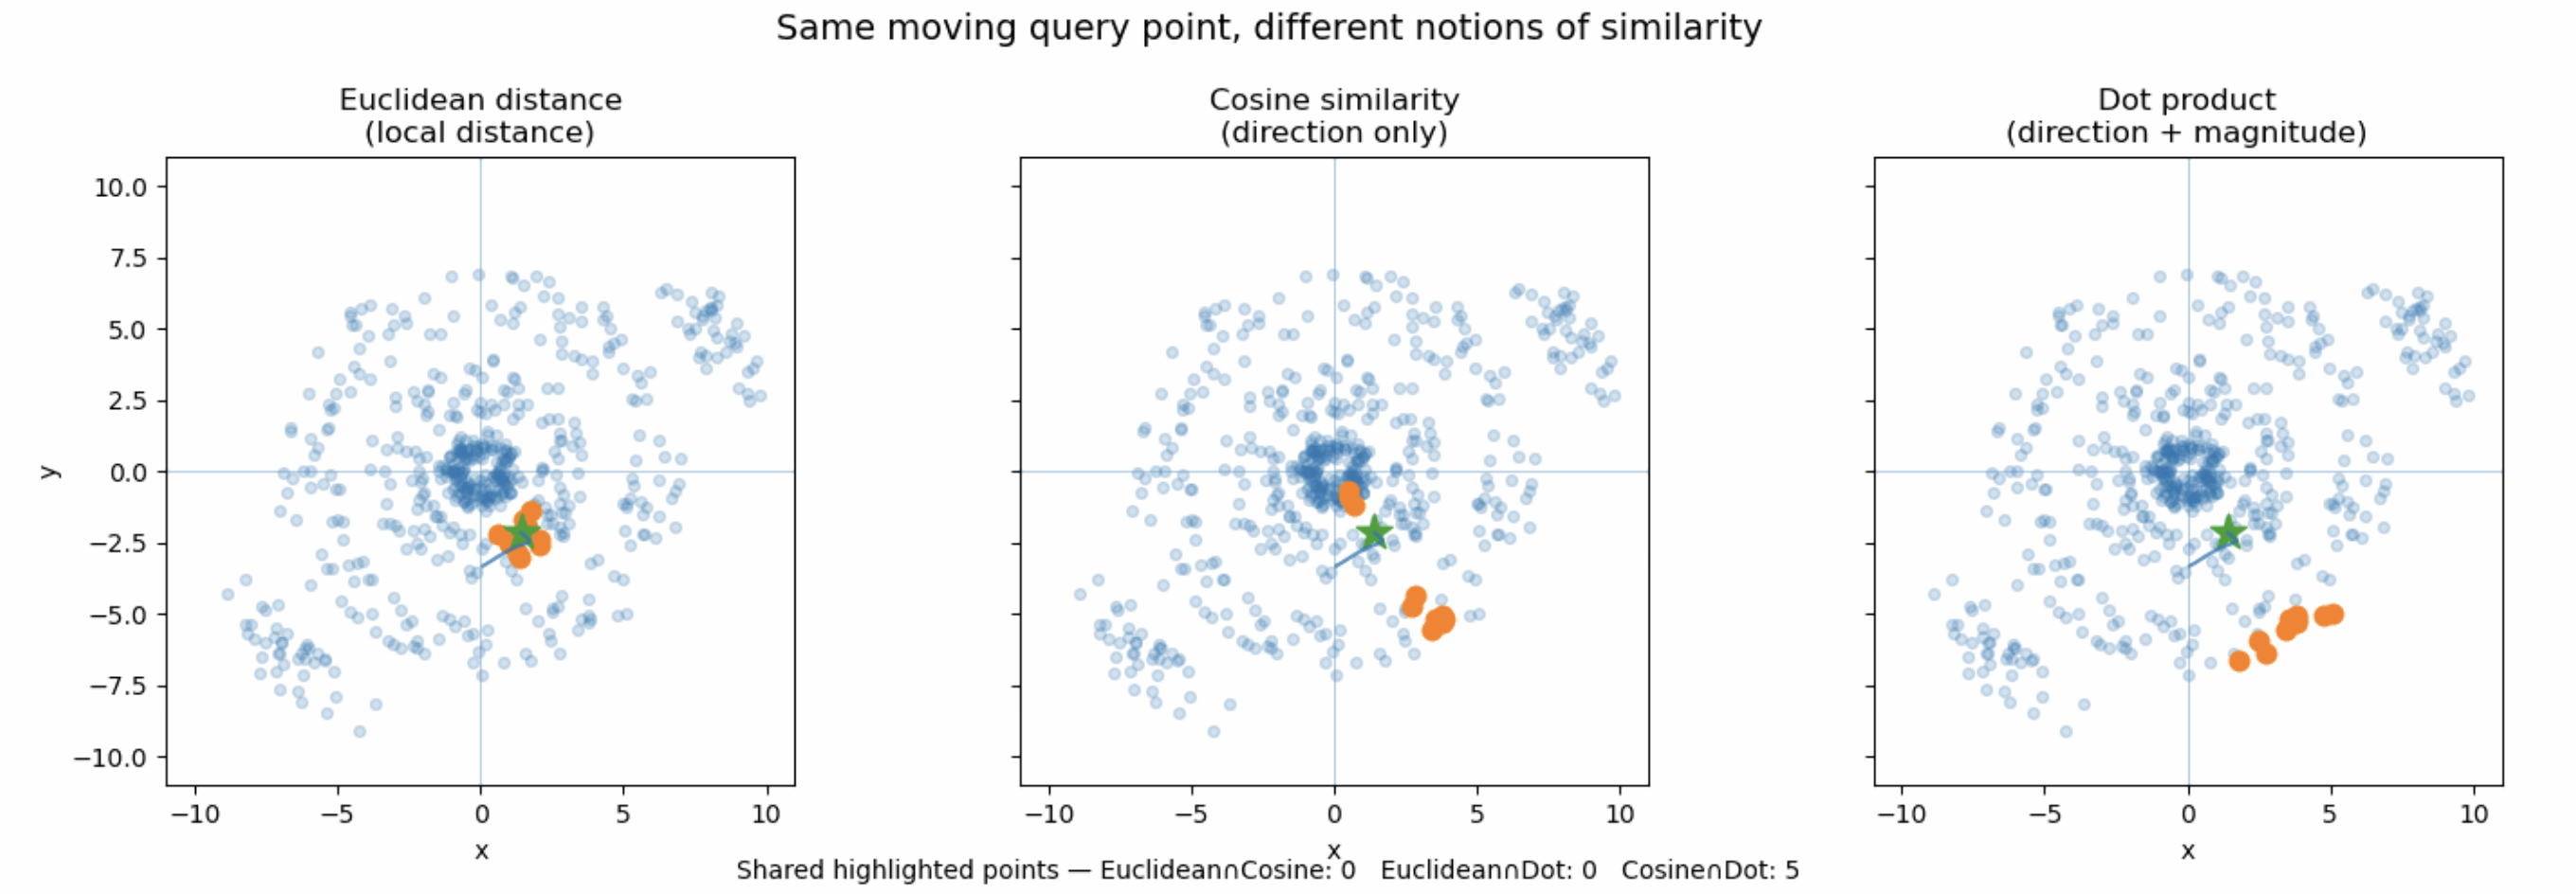
\includegraphics[width=1\linewidth, height=3cm]{dot_product_vs_consine.png}


\section{Content-Based Filtering}
\subsection{Methodology}
\smalltext{
we learn a weight vector and a bias term for each user using Ridge regression. The number of weights in the vector corresponds exactly to the number of item features (e.g., genres).
Construct user profiles based on historical item features. For each user $i$, train a regressor (e.g., \textbf{Ridge}) where $X$ is the feature matrix and $y$ are the user's ratings.
}
\subsection{Pros and Cons} 
\smalltext{ 
\textbf{Pros:} No item cold-start problem as brand-new movies can be recommended using metadata (genres, actors, etc.) even with zero ratings
; high transparency and interpretability because recommendations are easily explained via specific feature weights
; and user independence, ensuring that poor or biased data from other users does not impact an individual's profile. 
\textbf{Cons:} Significant user cold-start problem where users with sparse histories provide insufficient data for reliable modeling
; low serendipity as the system lacks the ability to suggest diverse genres, instead recommending "more of the same"
; and heavy dependency on high-quality metadata, as inaccurate or broad tags limit the model's predictive power}

\section{Implementation at Scale}
\subsection{Sparse Representations}
\smalltext{
Utility matrices for large sets are memory-prohibitive in dense formats. Using Compressed Sparse Row (\code{CSR}) formats stores only non-zero entries, reducing memory (e.g., 600GB dense $\rightarrow$ 8MB sparse).
}
\subsection{Data Modalities}
\smalltext{
\textbf{Explicit:} Direct feedback (ratings/likes). \textbf{Implicit:} Behavioral proxies (dwell time, click-through, purchase). Implicit data is more abundant but noisier.
}

\subsection{Evaluation Limitations}
\smalltext{
RMSE and MAE measure prediction accuracy but fail to capture user satisfaction. There is no single "ground truth" for preference.
}
\subsection{Optimization Dimensions}
\smalltext{
\begin{itemize}
    \item \textbf{Diversity:} Variance in recommendation categories.
    \item \textbf{Freshness/Serendipity:} Surprising or novel items.
    \item \textbf{Trust/Explainability:} Providing rationale for the suggestion.
    \item \textbf{Persistence:} Handling of ignored or decayed recommendations.
\end{itemize}
}

\end{multicols}
\end{document}